\subsection{Amortización y depreciación}

\subsubsection{Préstamo}

Para poner en marcha el proyecto, se gestionó un préstamo con una entidad bancaria, el cual se sumó al capital social de la empresa. La tabla \ref{prestamo} detalla la distribución de este capital en la compra de activos fijos necesarios, así como las condiciones del préstamo recibido.

\vspace{2mm}
\begin{minipage}{0.9\textwidth}
\centering
\captionof{table}[Préstamo]{Préstamo}
\label{prestamo}
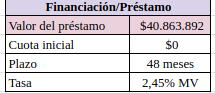
\includegraphics[width=0.6\textwidth]{Content/Images/AF/amortizacion_financiacion.png}
\footnote{Nota. \textup{Fuente: Autores}}
\end{minipage}

\subsubsection{Amortización}

A continuación, se muestra un resumen de los pagos anuales realizados. La tabla \ref{amortizacion} presenta la amortización total de la deuda, la cual está programada para ser saldada en un plazo de 4 años. En dicha tabla se especifica el cronograma de pagos, el saldo restante en cada periodo y los intereses aplicados, hasta que la deuda llegue a \$0.

\vspace{2mm}
\begin{minipage}{0.9\textwidth}
\centering
\captionof{table}[Amortización]{Amortización}
\label{amortizacion}
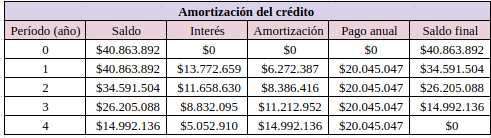
\includegraphics[width=0.6\textwidth]{Content/Images/AF/amortizacion_amortizacion.png}
\footnote{Nota. \textup{Fuente: Autores}}
\end{minipage}

\subsubsection{Depreciación}

La tabla \ref{depreciacion} muestra los equipos tecnológicos que se utilizarán en el proyecto, junto con la depreciación calculada por uso y obsolescencia. Se ha estimado una depreciación anual del 20\%, considerando una vida útil de 5 años para estos activos.

\vspace{2mm}
\begin{minipage}{0.9\textwidth}
\centering
\captionof{table}[Depreciación]{Depreciación}
\label{depreciacion}
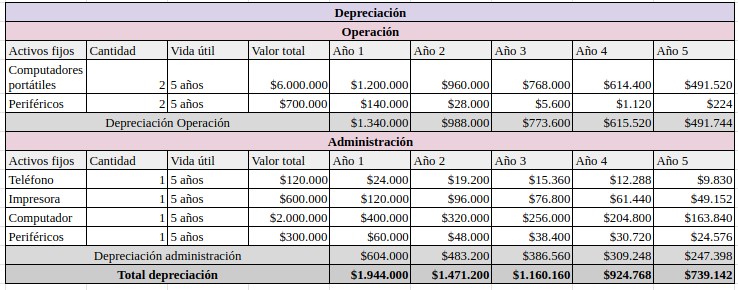
\includegraphics[width=0.6\textwidth]{Content/Images/AF/amortizacion_Depresiacion.png}
\footnote{Nota. \textup{Fuente: Autores}}
\end{minipage}
